
\begin{frame}{Classifier-Free Guidance}
	\small
	Để có thể học được có điều kiện (condition $c$).
	
	Với mỗi bước $t: T \rightarrow 1$, 
	\begin{columns}
		\begin{column}{0.6\textwidth}
			\begin{figure}
				\centering
				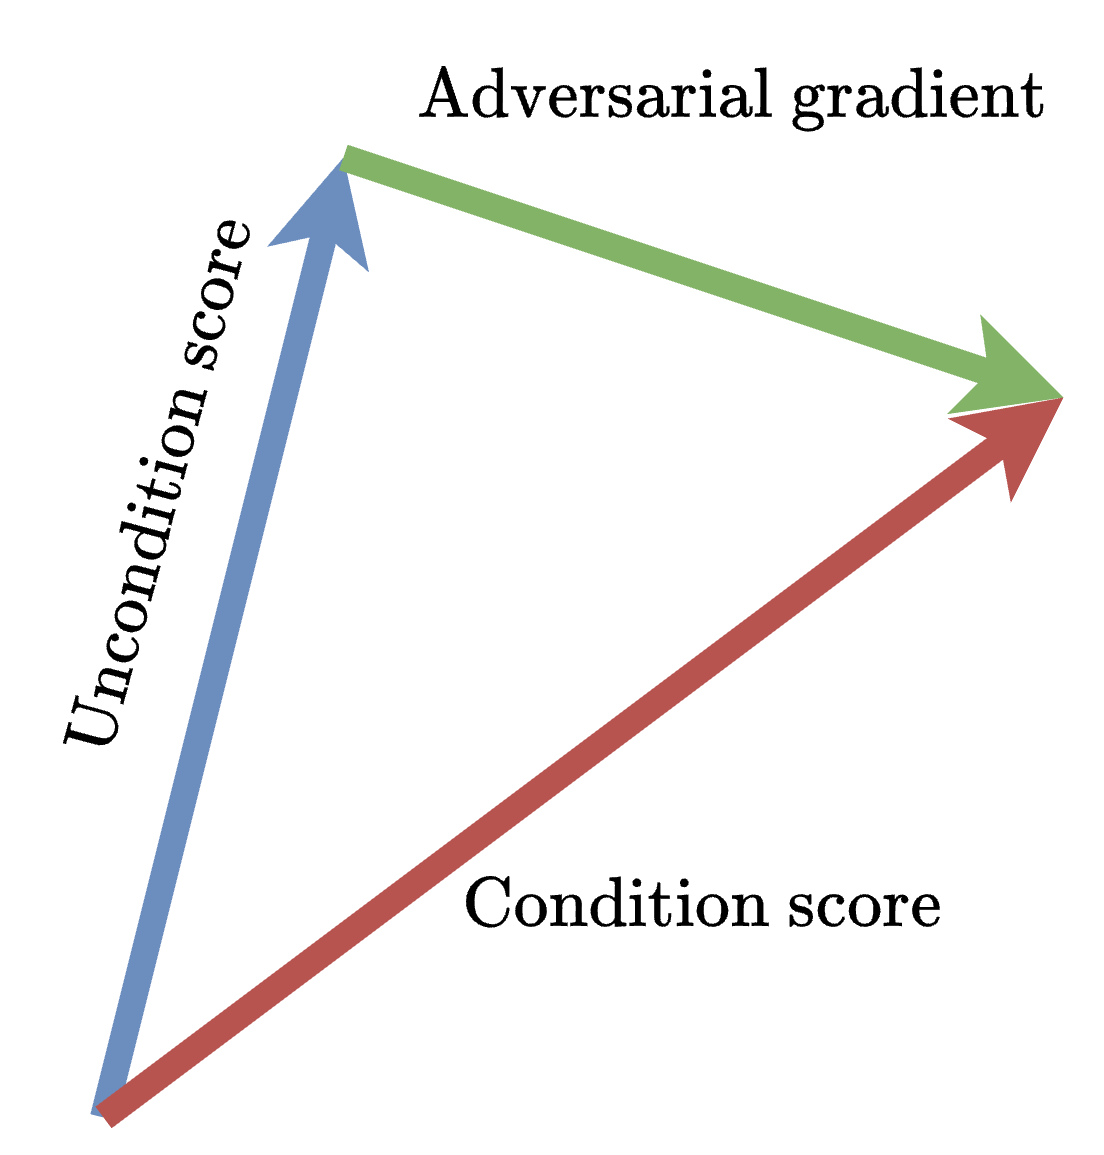
\includegraphics[width=0.45\linewidth]{Vector}
			\end{figure}
			{\footnotesize
			\begin{align*}
				\underbrace{\nabla \log p_{\gamma}(\bx_t | \by)}_{\text{Conditional score}} 
				&= \underbrace{\nabla \log p(\bx_t)}_{\text{Uncondition score}} + 
				\underbrace{\gamma \nabla \log p(\by | \bx_t)}_{\text{Adversarial gradient}} \\
				&= \underbrace{\nabla \log p(\bx_t)}_{\text{Uncondition score}} + 
				\underbrace{\gamma (\nabla \log p(\bx_t | \by) - \nabla \log p( \bx_t) )}_{\text{Adversarial gradient}} \\
				&= \underbrace{(1 - \gamma)\nabla \log p(\bx_t)}_{\text{Uncondition score}} + 
				\underbrace{\gamma \nabla \log p(\bx_t | \by)}_{\text{Condition score}}
			\end{align*}}
		
		\vspace{-15pt}
		\begin{equation*}
			\hat{\bx}_{0, \gamma, c} = \gamma f(\bx_t, t, c) + (1-\gamma) f (\bx_t, t, c_\varnothing)
		\end{equation*}
	
			
			
			
%			
%			\begin{align*}
%				\nabla_{\mathbf{x}_t} \log q(\mathbf{x}_t, y)
%				&= \nabla_{\mathbf{x}_t} \log q(\mathbf{x}_t) + \nabla_{\mathbf{x}_t} \log q(y \vert \mathbf{x}_t)		
%			\end{align*}
			
		\end{column}
		
		\begin{column}{0.4\textwidth}
			\begin{figure}
				\centering
				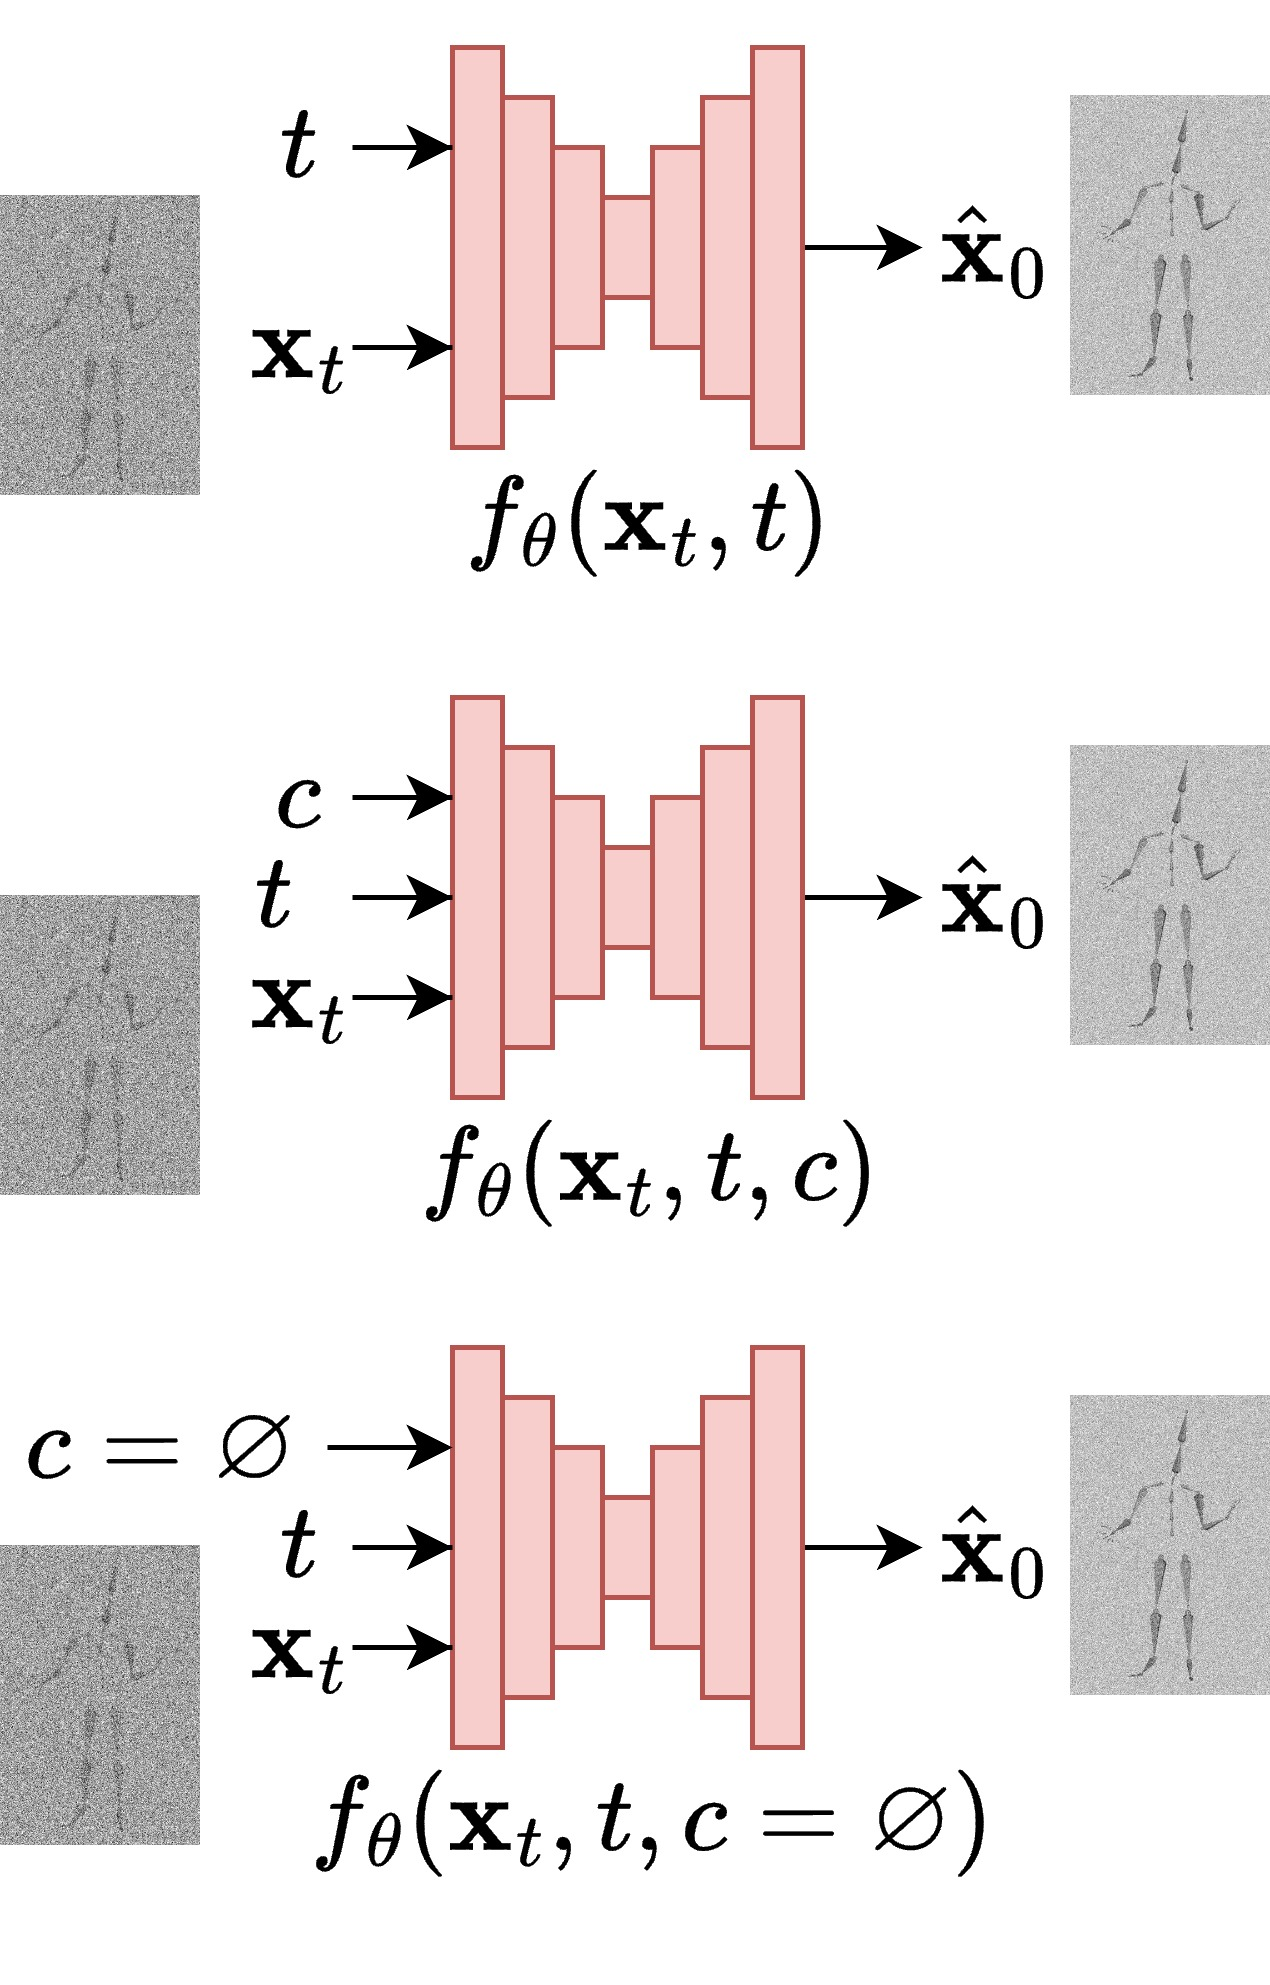
\includegraphics[width=\linewidth]{ConditionDiffusion}
			\end{figure}
		\end{column}
	\end{columns}
	
\end{frame}


\begin{frame}{Classifier-Free Guidance với $\mathbf{x}_0$ Objective}
	\begin{figure}
		\centering
		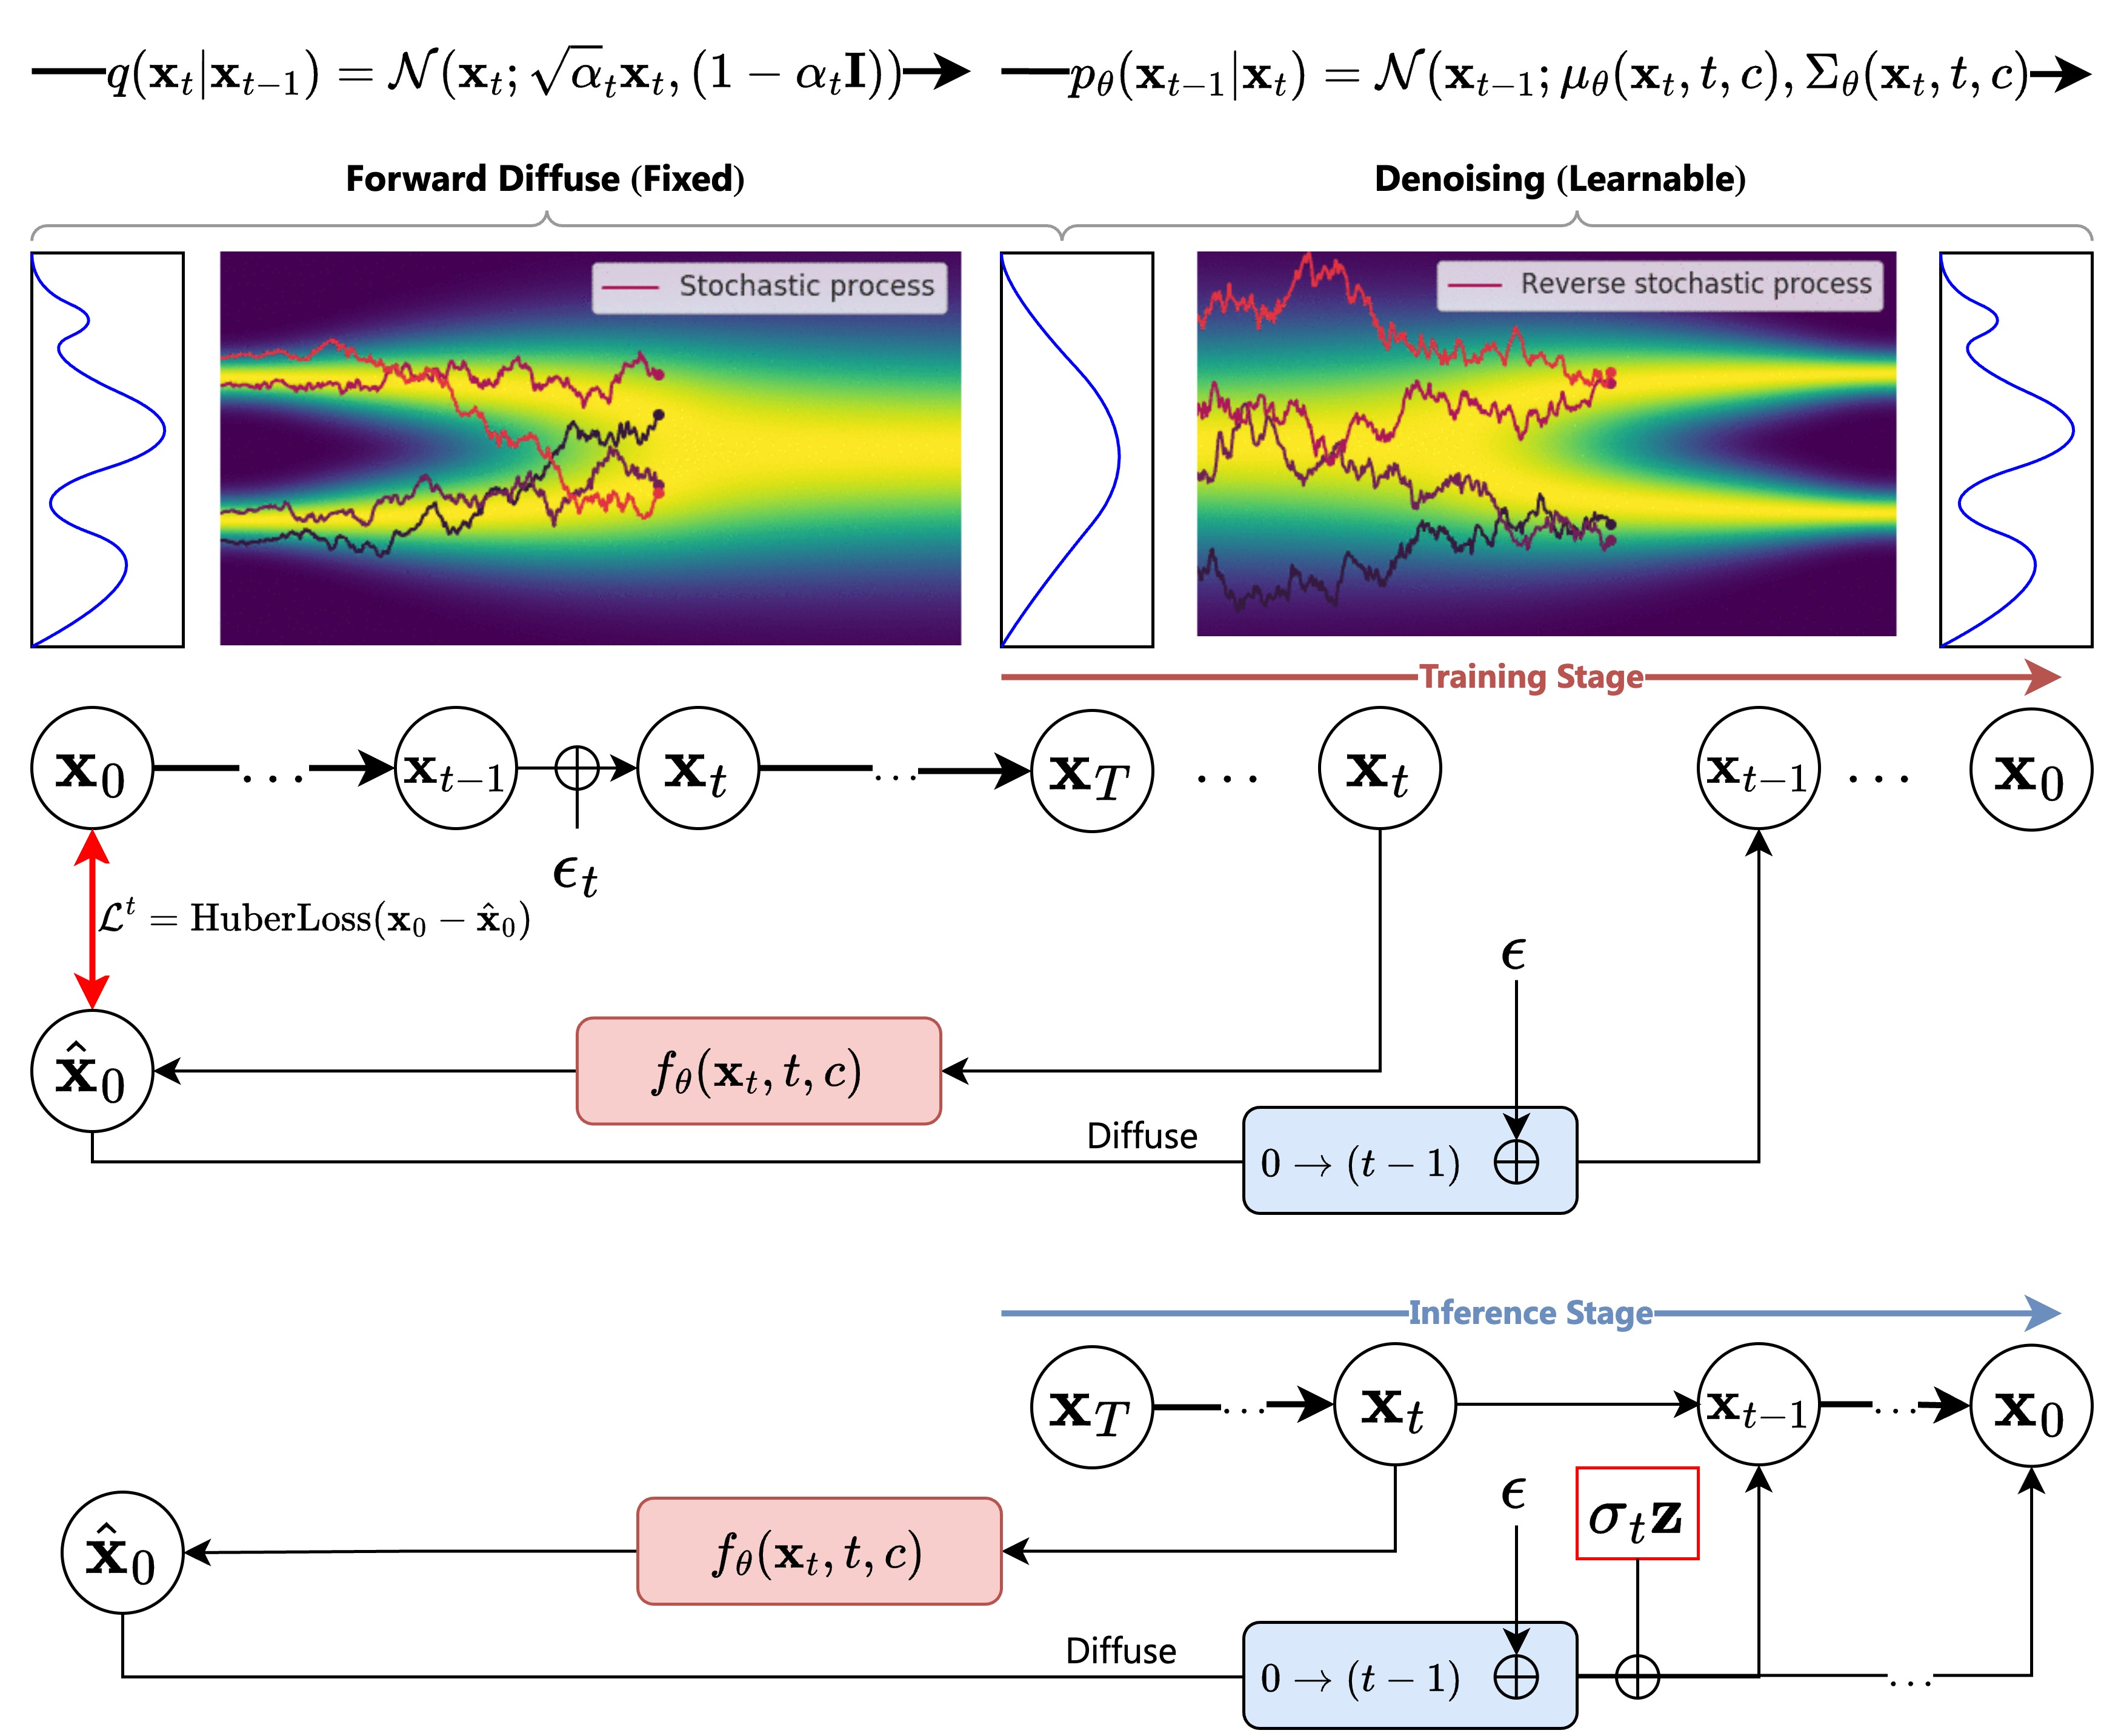
\includegraphics[width=0.95\linewidth]{TrainingAndSampling.jpg}
	\end{figure}
\end{frame}


